\documentclass{article}
\title{Probabilistic Graphical Models CS2950P HW1}
\author{Sam Boosalis (with Ryan Lester)}
\date{March 2013}



\usepackage[cm]{fullpage}
\usepackage{tikz}
\usepackage{verbatim}
\usepackage{parskip}

\usepackage{listings}


% read code from file and tex it up
% \lstinputlisting[]{../code.py}

% \usepackage[T1]{fontenc}
% \usepackage[scaled]{beramono}

%\lstset{
%  language=Python,
%  showstringspaces=false,
%  formfeed=\newpage,
%  tabsize=4,
%  commentstyle=\itshape,
%  basicstyle=\ttfamily,
%  morekeywords={G, lambda}
%}
%
%\newcommand{\code}[2]{
% \renewcommand*\familydefault{\ttdefault}
%
%  \hrulefill
%  \subsection*{#1}
%  \lstinputlisting{#2}
%  \vspace{2em}
%  
%}
%USAGE 
% \code{Python Code}{../code.py}


%\code{Python Code}{../theory.py}
%\code{Python Code}{../theory.py}

% 1.a 1.b 1.c ... (not 1.1 1.2 1.3 ...)
\renewcommand{\thesubsection}{\thesection.\alph{subsection}}

% \noindent everywhere
%\setlength{\parindent}{0pt}
%\setlength{\parsep}{1\baselineskip}
%\renewcommand{\indent}{\hspace*{10.95003pt}\ignorespaces}

% no
% \renewcommand{\paragraph}{\noindent \paragraph}

% underscores
% \def_{\_}




\begin{document}
\maketitle



\newpage
\section{Iterative Sum Product on Any Factor Graph}
\newpage

\subsection{}
(code in sumproduct.py and factorgraph.py and main.py)

\subsection{}
(code in sumproduct.py)

\subsection{}
(test by running ./sumproduct.py). \par
i first test on small graphs by explicitly passing messages. i then test both sum-product and brute-force on small factor trees by checking that the brute-force marginals equal manual solutions and by checking the algorithms against each other (equality is transitive). i test that the product of marginals of brute-force equal the product of right factors. i use variables of different dimensions, factors of different orders, and factors with different probabilities. i use a chain; a tree; a deeper binary tree; several variables and one factor; several factors and one variable; and a square with cycles. all the acyclic factor graphs converge within 10 iterations, and they all are exact (including the small cyclic graphs). the experimental evidence is to run $sumproduct.py$ and see the tests pass, which do the above.

\newpage

\subsubsection*{The Sum-Product Algorithm}
\lstinputlisting[]{../sumproduct.py}
\newpage

\subsubsection*{Port the Matlab to Python}
\lstinputlisting[]{../main.py}
\newpage
 
\subsubsection*{Port the Matlab to Python}
\lstinputlisting[]{../factorgraph.py}
\newpage



\newpage
\section{Inference on ALARM}
\newpage


\subsection{}
sumprod was exact
\newline mean PULMEMBOLUS = 1.99
\newline mean INTUBATION = 1.12999999822
\newline mean KINKEDTUBE = 1.96000000177
\newline mean VENTTUBE = 3.9400000013


\subsection{}
sumprod was exact
\newline mean PULMEMBOLUS = 1.98107225552
\newline mean INTUBATION = 2.90293067903
\newline mean KINKEDTUBE = 1.9985228765
\newline mean VENTTUBE = 3.92576957723


\subsection{}
sumprod was approx (VENTLUNG and INTUBATION are off by over 10\%)

[bruteforce means]
\newline mean VENTLUNG = 3.42842646489
\newline mean KINKEDTUBE = 1.99787701961
\newline mean INTUBATION = 1.54975162592
\newline mean VENTTUBE = 3.45951755981

[sumprod means]
\newline mean VENTLUNG = 2.66478879532
\newline mean KINKEDTUBE = 1.9931210537
\newline mean INTUBATION = 1.91289992443
\newline mean VENTTUBE = 3.43053893744


\subsection{}
% well, neither the subgraphs of (a), (b), or (c) are triangulated, due to the non-maximal / high-degree factors. \par

if we think of the factor graphs as just undirected graphs, all three have cycles. but if we only think about the variables communicating via factors, then the (c) subgraph has MINVOL, which makes a cycle between VENTLUNG and INTUBATION that propagates messages. this is consistent in that only VENTLUNG and INTUBATION are significantly different from their exact values.
 
\subsection{}
sumprod probably computes inexact marginals. the graph has too many variable cycles.

[sumprod: converged (eps=1e-06) in 14 iterations]
\newline mean DISCONNECT = 1.9
\newline mean PULMEMBOLUS = 1.99001429995
\newline mean INSUFFANESTH = 1.90043976042
\newline mean LVFAILURE = 1.95
\newline mean ANAPHYLAXIS = 1.99106463727

\subsection{}
i don't think these estimates coincide with the true means. 

[sumprod: converged (eps=1e-06) in 24 iterations]
\newline mean DISCONNECT = 1.90000000337
\newline mean HYPOVOLEMIA = 1.8
\newline mean LVFAILURE = 1.95
\newline mean KINKEDTUBE = 1.9600000015
\newline mean INTUBATION = 1.12999999528
\newline mean INSUFFANESTH = 1.9
\newline mean ANAPHYLAXIS = 1.99
\newline mean PULMEMBOLUS = 1.99

\subsection{}
[sumprod: iterated too many times (N=500) with (diff=0.576824503)]
\newline mean DISCONNECT	=	1.9046026259
\newline mean HYPOVOLEMIA	=	1.8022572855
\newline mean LVFAILURE	=	1.00455640119
\newline mean KINKEDTUBE	=	1.95330338292
\newline mean INTUBATION	=	1.21543803025
\newline mean INSUFFANESTH	=	1.90640901319
\newline mean ANAPHYLAXIS	=	1.99181228874
\newline mean PULMEMBOLUS	=	1.99059265509


\subsection{}
the only significant difference between the means of (g) and (h) is INTUBATION, differing by over 10\%. this makes sense as INTUBATION is in the most factors of any of the diagnostic variables. \par
the most significant difference is that (h) converges whereas (g) doesn't.

[sumprod: converged (eps=1e-06) in 289 iterations]
\newline mean DISCONNECT	=	1.89900334967
\newline mean HYPOVOLEMIA	=	1.80280398577
\newline mean LVFAILURE	=	1.00519005918
\newline mean KINKEDTUBE	=	1.96375990063
\newline mean INTUBATION	=	1.46785783435
\newline mean INSUFFANESTH	=	1.8986736855
\newline mean ANAPHYLAXIS	=	1.98457027707
\newline mean PULMEMBOLUS	=	1.9899078908




\newpage
\subsection*{ALARM}
\lstinputlisting[]{../alarm.py}
\newpage



\newpage
\section{Elimination on 2D Grids}
\newpage

%TODO
%\begin{comment}


\subsection{}
the maximal elimination clique is 5 once we eliminate $(2)$ (the graph gets connected and stays connected).

\begin{center}
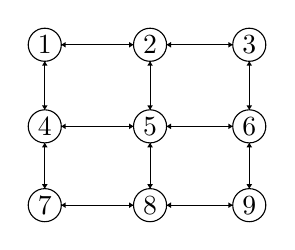
\begin{tikzpicture}[scale=0.07]
\tikzstyle{every node}+=[inner sep=0pt]
\draw [black] (18.7,-10.9) circle (3);
\draw (18.7,-10.9) node {$1$};
\draw [black] (37.8,-10.9) circle (3);
\draw (37.8,-10.9) node {$2$};
\draw [black] (55.8,-10.9) circle (3);
\draw (55.8,-10.9) node {$3$};
\draw [black] (18.7,-25.7) circle (3);
\draw (18.7,-25.7) node {$4$};
\draw [black] (18.7,-40) circle (3);
\draw (18.7,-40) node {$7$};
\draw [black] (37.8,-25.7) circle (3);
\draw (37.8,-25.7) node {$5$};
\draw [black] (55.8,-25.7) circle (3);
\draw (55.8,-25.7) node {$6$};
\draw [black] (37.8,-40) circle (3);
\draw (37.8,-40) node {$8$};
\draw [black] (55.8,-40) circle (3);
\draw (55.8,-40) node {$9$};
\draw [black] (21.7,-10.9) -- (34.8,-10.9);
\fill [black] (34.8,-10.9) -- (34,-10.4) -- (34,-11.4);
\draw [black] (34.8,-10.9) -- (21.7,-10.9);
\fill [black] (21.7,-10.9) -- (22.5,-11.4) -- (22.5,-10.4);
\draw [black] (18.7,-13.9) -- (18.7,-22.7);
\fill [black] (18.7,-22.7) -- (19.2,-21.9) -- (18.2,-21.9);
\draw [black] (21.7,-25.7) -- (34.8,-25.7);
\fill [black] (34.8,-25.7) -- (34,-25.2) -- (34,-26.2);
\draw [black] (34.8,-25.7) -- (21.7,-25.7);
\fill [black] (21.7,-25.7) -- (22.5,-26.2) -- (22.5,-25.2);
\draw [black] (18.7,-22.7) -- (18.7,-13.9);
\fill [black] (18.7,-13.9) -- (18.2,-14.7) -- (19.2,-14.7);
\draw [black] (18.7,-28.7) -- (18.7,-37);
\fill [black] (18.7,-37) -- (19.2,-36.2) -- (18.2,-36.2);
\draw [black] (18.7,-37) -- (18.7,-28.7);
\fill [black] (18.7,-28.7) -- (18.2,-29.5) -- (19.2,-29.5);
\draw [black] (37.8,-28.7) -- (37.8,-37);
\fill [black] (37.8,-37) -- (38.3,-36.2) -- (37.3,-36.2);
\draw [black] (37.8,-37) -- (37.8,-28.7);
\fill [black] (37.8,-28.7) -- (37.3,-29.5) -- (38.3,-29.5);
\draw [black] (52.8,-25.7) -- (40.8,-25.7);
\fill [black] (40.8,-25.7) -- (41.6,-26.2) -- (41.6,-25.2);
\draw [black] (40.8,-25.7) -- (52.8,-25.7);
\fill [black] (52.8,-25.7) -- (52,-25.2) -- (52,-26.2);
\draw [black] (21.7,-40) -- (34.8,-40);
\fill [black] (34.8,-40) -- (34,-39.5) -- (34,-40.5);
\draw [black] (34.8,-40) -- (21.7,-40);
\fill [black] (21.7,-40) -- (22.5,-40.5) -- (22.5,-39.5);
\draw [black] (40.8,-40) -- (52.8,-40);
\fill [black] (52.8,-40) -- (52,-39.5) -- (52,-40.5);
\draw [black] (52.8,-40) -- (40.8,-40);
\fill [black] (40.8,-40) -- (41.6,-40.5) -- (41.6,-39.5);
\draw [black] (55.8,-28.7) -- (55.8,-37);
\fill [black] (55.8,-37) -- (56.3,-36.2) -- (55.3,-36.2);
\draw [black] (55.8,-37) -- (55.8,-28.7);
\fill [black] (55.8,-28.7) -- (55.3,-29.5) -- (56.3,-29.5);
\draw [black] (55.8,-22.7) -- (55.8,-13.9);
\fill [black] (55.8,-13.9) -- (55.3,-14.7) -- (56.3,-14.7);
\draw [black] (55.8,-13.9) -- (55.8,-22.7);
\fill [black] (55.8,-22.7) -- (56.3,-21.9) -- (55.3,-21.9);
\draw [black] (52.8,-10.9) -- (40.8,-10.9);
\fill [black] (40.8,-10.9) -- (41.6,-11.4) -- (41.6,-10.4);
\draw [black] (37.8,-22.7) -- (37.8,-13.9);
\fill [black] (37.8,-13.9) -- (37.3,-14.7) -- (38.3,-14.7);
\draw [black] (37.8,-13.9) -- (37.8,-22.7);
\fill [black] (37.8,-22.7) -- (38.3,-21.9) -- (37.3,-21.9);
\draw [black] (40.8,-10.9) -- (52.8,-10.9);
\fill [black] (52.8,-10.9) -- (52,-10.4) -- (52,-11.4);
\end{tikzpicture}
\end{center}



\begin{center}
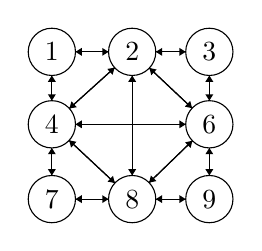
\begin{tikzpicture}[scale=0.1]
\tikzstyle{every node}+=[inner sep=0pt]
\draw [black] (28.4,-13.8) circle (3);
\draw (28.4,-13.8) node {$2$};
\draw [black] (38.2,-13.8) circle (3);
\draw (38.2,-13.8) node {$3$};
\draw [black] (18.2,-23) circle (3);
\draw (18.2,-23) node {$4$};
\draw [black] (38.2,-23) circle (3);
\draw (38.2,-23) node {$6$};
\draw [black] (18.2,-32.5) circle (3);
\draw (18.2,-32.5) node {$7$};
\draw [black] (28.4,-32.5) circle (3);
\draw (28.4,-32.5) node {$8$};
\draw [black] (38.2,-32.5) circle (3);
\draw (38.2,-32.5) node {$9$};
\draw [black] (18.2,-13.8) circle (3);
\draw (18.2,-13.8) node {$1$};
\draw [black] (36.01,-20.95) -- (30.59,-15.85);
\fill [black] (30.59,-15.85) -- (30.83,-16.77) -- (31.51,-16.04);
\draw [black] (30.59,-15.85) -- (36.01,-20.95);
\fill [black] (36.01,-20.95) -- (35.77,-20.03) -- (35.09,-20.76);
\draw [black] (38.2,-20) -- (38.2,-16.8);
\fill [black] (38.2,-16.8) -- (37.7,-17.6) -- (38.7,-17.6);
\draw [black] (38.2,-16.8) -- (38.2,-20);
\fill [black] (38.2,-20) -- (38.7,-19.2) -- (37.7,-19.2);
\draw [black] (38.2,-26) -- (38.2,-29.5);
\fill [black] (38.2,-29.5) -- (38.7,-28.7) -- (37.7,-28.7);
\draw [black] (38.2,-29.5) -- (38.2,-26);
\fill [black] (38.2,-26) -- (37.7,-26.8) -- (38.7,-26.8);
\draw [black] (35.2,-13.8) -- (31.4,-13.8);
\fill [black] (31.4,-13.8) -- (32.2,-14.3) -- (32.2,-13.3);
\draw [black] (31.4,-13.8) -- (35.2,-13.8);
\fill [black] (35.2,-13.8) -- (34.4,-13.3) -- (34.4,-14.3);
\draw [black] (26.17,-15.81) -- (20.43,-20.99);
\fill [black] (20.43,-20.99) -- (21.36,-20.83) -- (20.69,-20.08);
\draw [black] (20.43,-20.99) -- (26.17,-15.81);
\fill [black] (26.17,-15.81) -- (25.24,-15.97) -- (25.91,-16.72);
\draw [black] (18.2,-26) -- (18.2,-29.5);
\fill [black] (18.2,-29.5) -- (18.7,-28.7) -- (17.7,-28.7);
\draw [black] (18.2,-29.5) -- (18.2,-26);
\fill [black] (18.2,-26) -- (17.7,-26.8) -- (18.7,-26.8);
\draw [black] (21.2,-32.5) -- (25.4,-32.5);
\fill [black] (25.4,-32.5) -- (24.6,-32) -- (24.6,-33);
\draw [black] (25.4,-32.5) -- (21.2,-32.5);
\fill [black] (21.2,-32.5) -- (22,-33) -- (22,-32);
\draw [black] (31.4,-32.5) -- (35.2,-32.5);
\fill [black] (35.2,-32.5) -- (34.4,-32) -- (34.4,-33);
\draw [black] (35.2,-32.5) -- (31.4,-32.5);
\fill [black] (31.4,-32.5) -- (32.2,-33) -- (32.2,-32);
\draw [black] (30.55,-30.41) -- (36.05,-25.09);
\fill [black] (36.05,-25.09) -- (35.12,-25.29) -- (35.82,-26);
\draw [black] (36.05,-25.09) -- (30.55,-30.41);
\fill [black] (30.55,-30.41) -- (31.48,-30.21) -- (30.78,-29.5);
\draw [black] (26.2,-30.46) -- (20.4,-25.04);
\fill [black] (20.4,-25.04) -- (20.64,-25.96) -- (21.32,-25.22);
\draw [black] (20.4,-25.04) -- (26.2,-30.46);
\fill [black] (26.2,-30.46) -- (25.96,-29.54) -- (25.28,-30.28);
\draw [black] (21.2,-23) -- (35.2,-23);
\fill [black] (35.2,-23) -- (34.4,-22.5) -- (34.4,-23.5);
\draw [black] (35.2,-23) -- (21.2,-23);
\fill [black] (21.2,-23) -- (22,-23.5) -- (22,-22.5);
\draw [black] (28.4,-29.5) -- (28.4,-16.8);
\fill [black] (28.4,-16.8) -- (27.9,-17.6) -- (28.9,-17.6);
\draw [black] (28.4,-16.8) -- (28.4,-29.5);
\fill [black] (28.4,-29.5) -- (28.9,-28.7) -- (27.9,-28.7);
\draw [black] (18.2,-20) -- (18.2,-16.8);
\fill [black] (18.2,-16.8) -- (17.7,-17.6) -- (18.7,-17.6);
\draw [black] (18.2,-16.8) -- (18.2,-20);
\fill [black] (18.2,-20) -- (18.7,-19.2) -- (17.7,-19.2);
\draw [black] (21.2,-13.8) -- (25.4,-13.8);
\fill [black] (25.4,-13.8) -- (24.6,-13.3) -- (24.6,-14.3);
\draw [black] (25.4,-13.8) -- (21.2,-13.8);
\fill [black] (21.2,-13.8) -- (22,-14.3) -- (22,-13.3);
\end{tikzpicture}
\end{center}



\begin{center}
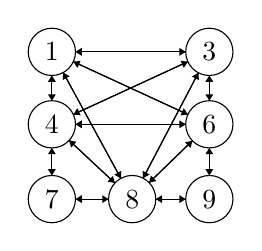
\begin{tikzpicture}[scale=0.1]
\tikzstyle{every node}+=[inner sep=0pt]
\draw [black] (38.2,-13.8) circle (3);
\draw (38.2,-13.8) node {$3$};
\draw [black] (18.2,-23) circle (3);
\draw (18.2,-23) node {$4$};
\draw [black] (38.2,-23) circle (3);
\draw (38.2,-23) node {$6$};
\draw [black] (18.2,-32.5) circle (3);
\draw (18.2,-32.5) node {$7$};
\draw [black] (28.4,-32.5) circle (3);
\draw (28.4,-32.5) node {$8$};
\draw [black] (38.2,-32.5) circle (3);
\draw (38.2,-32.5) node {$9$};
\draw [black] (18.2,-13.8) circle (3);
\draw (18.2,-13.8) node {$1$};
\draw [black] (38.2,-20) -- (38.2,-16.8);
\fill [black] (38.2,-16.8) -- (37.7,-17.6) -- (38.7,-17.6);
\draw [black] (38.2,-16.8) -- (38.2,-20);
\fill [black] (38.2,-20) -- (38.7,-19.2) -- (37.7,-19.2);
\draw [black] (38.2,-26) -- (38.2,-29.5);
\fill [black] (38.2,-29.5) -- (38.7,-28.7) -- (37.7,-28.7);
\draw [black] (38.2,-29.5) -- (38.2,-26);
\fill [black] (38.2,-26) -- (37.7,-26.8) -- (38.7,-26.8);
\draw [black] (18.2,-26) -- (18.2,-29.5);
\fill [black] (18.2,-29.5) -- (18.7,-28.7) -- (17.7,-28.7);
\draw [black] (18.2,-29.5) -- (18.2,-26);
\fill [black] (18.2,-26) -- (17.7,-26.8) -- (18.7,-26.8);
\draw [black] (21.2,-32.5) -- (25.4,-32.5);
\fill [black] (25.4,-32.5) -- (24.6,-32) -- (24.6,-33);
\draw [black] (25.4,-32.5) -- (21.2,-32.5);
\fill [black] (21.2,-32.5) -- (22,-33) -- (22,-32);
\draw [black] (31.4,-32.5) -- (35.2,-32.5);
\fill [black] (35.2,-32.5) -- (34.4,-32) -- (34.4,-33);
\draw [black] (35.2,-32.5) -- (31.4,-32.5);
\fill [black] (31.4,-32.5) -- (32.2,-33) -- (32.2,-32);
\draw [black] (30.55,-30.41) -- (36.05,-25.09);
\fill [black] (36.05,-25.09) -- (35.12,-25.29) -- (35.82,-26);
\draw [black] (36.05,-25.09) -- (30.55,-30.41);
\fill [black] (30.55,-30.41) -- (31.48,-30.21) -- (30.78,-29.5);
\draw [black] (26.2,-30.46) -- (20.4,-25.04);
\fill [black] (20.4,-25.04) -- (20.64,-25.96) -- (21.32,-25.22);
\draw [black] (20.4,-25.04) -- (26.2,-30.46);
\fill [black] (26.2,-30.46) -- (25.96,-29.54) -- (25.28,-30.28);
\draw [black] (21.2,-23) -- (35.2,-23);
\fill [black] (35.2,-23) -- (34.4,-22.5) -- (34.4,-23.5);
\draw [black] (35.2,-23) -- (21.2,-23);
\fill [black] (21.2,-23) -- (22,-23.5) -- (22,-22.5);
\draw [black] (18.2,-20) -- (18.2,-16.8);
\fill [black] (18.2,-16.8) -- (17.7,-17.6) -- (18.7,-17.6);
\draw [black] (18.2,-16.8) -- (18.2,-20);
\fill [black] (18.2,-20) -- (18.7,-19.2) -- (17.7,-19.2);
\draw [black] (26.96,-29.87) -- (19.64,-16.43);
\fill [black] (19.64,-16.43) -- (19.58,-17.38) -- (20.46,-16.9);
\draw [black] (19.64,-16.43) -- (26.96,-29.87);
\fill [black] (26.96,-29.87) -- (27.02,-28.92) -- (26.14,-29.4);
\draw [black] (29.79,-29.84) -- (36.81,-16.46);
\fill [black] (36.81,-16.46) -- (35.99,-16.93) -- (36.88,-17.4);
\draw [black] (36.81,-16.46) -- (29.79,-29.84);
\fill [black] (29.79,-29.84) -- (30.61,-29.37) -- (29.72,-28.9);
\draw [black] (21.2,-13.8) -- (35.2,-13.8);
\fill [black] (35.2,-13.8) -- (34.4,-13.3) -- (34.4,-14.3);
\draw [black] (35.2,-13.8) -- (21.2,-13.8);
\fill [black] (21.2,-13.8) -- (22,-14.3) -- (22,-13.3);
\draw [black] (35.47,-21.75) -- (20.93,-15.05);
\fill [black] (20.93,-15.05) -- (21.44,-15.84) -- (21.86,-14.93);
\draw [black] (20.93,-15.05) -- (35.47,-21.75);
\fill [black] (35.47,-21.75) -- (34.96,-20.96) -- (34.54,-21.87);
\draw [black] (20.93,-21.75) -- (35.47,-15.05);
\fill [black] (35.47,-15.05) -- (34.54,-14.93) -- (34.96,-15.84);
\draw [black] (35.47,-15.05) -- (20.93,-21.75);
\fill [black] (20.93,-21.75) -- (21.86,-21.87) -- (21.44,-20.96);
\end{tikzpicture}
\end{center}




\begin{center}
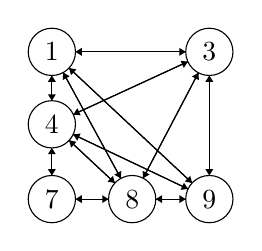
\begin{tikzpicture}[scale=0.1]
\tikzstyle{every node}+=[inner sep=0pt]
\draw [black] (38.2,-13.8) circle (3);
\draw (38.2,-13.8) node {$3$};
\draw [black] (18.2,-23) circle (3);
\draw (18.2,-23) node {$4$};
\draw [black] (18.2,-32.5) circle (3);
\draw (18.2,-32.5) node {$7$};
\draw [black] (28.4,-32.5) circle (3);
\draw (28.4,-32.5) node {$8$};
\draw [black] (38.2,-32.5) circle (3);
\draw (38.2,-32.5) node {$9$};
\draw [black] (18.2,-13.8) circle (3);
\draw (18.2,-13.8) node {$1$};
\draw [black] (18.2,-26) -- (18.2,-29.5);
\fill [black] (18.2,-29.5) -- (18.7,-28.7) -- (17.7,-28.7);
\draw [black] (18.2,-29.5) -- (18.2,-26);
\fill [black] (18.2,-26) -- (17.7,-26.8) -- (18.7,-26.8);
\draw [black] (21.2,-32.5) -- (25.4,-32.5);
\fill [black] (25.4,-32.5) -- (24.6,-32) -- (24.6,-33);
\draw [black] (25.4,-32.5) -- (21.2,-32.5);
\fill [black] (21.2,-32.5) -- (22,-33) -- (22,-32);
\draw [black] (31.4,-32.5) -- (35.2,-32.5);
\fill [black] (35.2,-32.5) -- (34.4,-32) -- (34.4,-33);
\draw [black] (35.2,-32.5) -- (31.4,-32.5);
\fill [black] (31.4,-32.5) -- (32.2,-33) -- (32.2,-32);
\draw [black] (26.2,-30.46) -- (20.4,-25.04);
\fill [black] (20.4,-25.04) -- (20.64,-25.96) -- (21.32,-25.22);
\draw [black] (20.4,-25.04) -- (26.2,-30.46);
\fill [black] (26.2,-30.46) -- (25.96,-29.54) -- (25.28,-30.28);
\draw [black] (18.2,-20) -- (18.2,-16.8);
\fill [black] (18.2,-16.8) -- (17.7,-17.6) -- (18.7,-17.6);
\draw [black] (18.2,-16.8) -- (18.2,-20);
\fill [black] (18.2,-20) -- (18.7,-19.2) -- (17.7,-19.2);
\draw [black] (26.96,-29.87) -- (19.64,-16.43);
\fill [black] (19.64,-16.43) -- (19.58,-17.38) -- (20.46,-16.9);
\draw [black] (19.64,-16.43) -- (26.96,-29.87);
\fill [black] (26.96,-29.87) -- (27.02,-28.92) -- (26.14,-29.4);
\draw [black] (29.79,-29.84) -- (36.81,-16.46);
\fill [black] (36.81,-16.46) -- (35.99,-16.93) -- (36.88,-17.4);
\draw [black] (36.81,-16.46) -- (29.79,-29.84);
\fill [black] (29.79,-29.84) -- (30.61,-29.37) -- (29.72,-28.9);
\draw [black] (21.2,-13.8) -- (35.2,-13.8);
\fill [black] (35.2,-13.8) -- (34.4,-13.3) -- (34.4,-14.3);
\draw [black] (35.2,-13.8) -- (21.2,-13.8);
\fill [black] (21.2,-13.8) -- (22,-14.3) -- (22,-13.3);
\draw [black] (20.93,-21.75) -- (35.47,-15.05);
\fill [black] (35.47,-15.05) -- (34.54,-14.93) -- (34.96,-15.84);
\draw [black] (35.47,-15.05) -- (20.93,-21.75);
\fill [black] (20.93,-21.75) -- (21.86,-21.87) -- (21.44,-20.96);
\draw [black] (36.01,-30.45) -- (20.39,-15.85);
\fill [black] (20.39,-15.85) -- (20.63,-16.76) -- (21.32,-16.03);
\draw [black] (20.39,-15.85) -- (36.01,-30.45);
\fill [black] (36.01,-30.45) -- (35.77,-29.54) -- (35.08,-30.27);
\draw [black] (38.2,-29.5) -- (38.2,-16.8);
\fill [black] (38.2,-16.8) -- (37.7,-17.6) -- (38.7,-17.6);
\draw [black] (38.2,-16.8) -- (38.2,-29.5);
\fill [black] (38.2,-29.5) -- (38.7,-28.7) -- (37.7,-28.7);
\draw [black] (20.91,-24.29) -- (35.49,-31.21);
\fill [black] (35.49,-31.21) -- (34.98,-30.42) -- (34.55,-31.32);
\draw [black] (35.49,-31.21) -- (20.91,-24.29);
\fill [black] (20.91,-24.29) -- (21.42,-25.08) -- (21.85,-24.18);
\end{tikzpicture}
\end{center}




\begin{center}
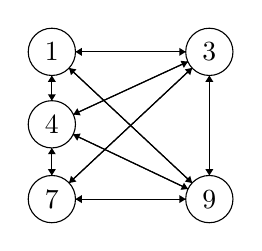
\begin{tikzpicture}[scale=0.1]
\tikzstyle{every node}+=[inner sep=0pt]
\draw [black] (38.2,-13.8) circle (3);
\draw (38.2,-13.8) node {$3$};
\draw [black] (18.2,-23) circle (3);
\draw (18.2,-23) node {$4$};
\draw [black] (18.2,-32.5) circle (3);
\draw (18.2,-32.5) node {$7$};
\draw [black] (38.2,-32.5) circle (3);
\draw (38.2,-32.5) node {$9$};
\draw [black] (18.2,-13.8) circle (3);
\draw (18.2,-13.8) node {$1$};
\draw [black] (18.2,-26) -- (18.2,-29.5);
\fill [black] (18.2,-29.5) -- (18.7,-28.7) -- (17.7,-28.7);
\draw [black] (18.2,-29.5) -- (18.2,-26);
\fill [black] (18.2,-26) -- (17.7,-26.8) -- (18.7,-26.8);
\draw [black] (18.2,-20) -- (18.2,-16.8);
\fill [black] (18.2,-16.8) -- (17.7,-17.6) -- (18.7,-17.6);
\draw [black] (18.2,-16.8) -- (18.2,-20);
\fill [black] (18.2,-20) -- (18.7,-19.2) -- (17.7,-19.2);
\draw [black] (21.2,-13.8) -- (35.2,-13.8);
\fill [black] (35.2,-13.8) -- (34.4,-13.3) -- (34.4,-14.3);
\draw [black] (35.2,-13.8) -- (21.2,-13.8);
\fill [black] (21.2,-13.8) -- (22,-14.3) -- (22,-13.3);
\draw [black] (20.93,-21.75) -- (35.47,-15.05);
\fill [black] (35.47,-15.05) -- (34.54,-14.93) -- (34.96,-15.84);
\draw [black] (35.47,-15.05) -- (20.93,-21.75);
\fill [black] (20.93,-21.75) -- (21.86,-21.87) -- (21.44,-20.96);
\draw [black] (36.01,-30.45) -- (20.39,-15.85);
\fill [black] (20.39,-15.85) -- (20.63,-16.76) -- (21.32,-16.03);
\draw [black] (20.39,-15.85) -- (36.01,-30.45);
\fill [black] (36.01,-30.45) -- (35.77,-29.54) -- (35.08,-30.27);
\draw [black] (38.2,-29.5) -- (38.2,-16.8);
\fill [black] (38.2,-16.8) -- (37.7,-17.6) -- (38.7,-17.6);
\draw [black] (38.2,-16.8) -- (38.2,-29.5);
\fill [black] (38.2,-29.5) -- (38.7,-28.7) -- (37.7,-28.7);
\draw [black] (20.91,-24.29) -- (35.49,-31.21);
\fill [black] (35.49,-31.21) -- (34.98,-30.42) -- (34.55,-31.32);
\draw [black] (35.49,-31.21) -- (20.91,-24.29);
\fill [black] (20.91,-24.29) -- (21.42,-25.08) -- (21.85,-24.18);
\draw [black] (21.2,-32.5) -- (35.2,-32.5);
\fill [black] (35.2,-32.5) -- (34.4,-32) -- (34.4,-33);
\draw [black] (35.2,-32.5) -- (21.2,-32.5);
\fill [black] (21.2,-32.5) -- (22,-33) -- (22,-32);
\draw [black] (20.39,-30.45) -- (36.01,-15.85);
\fill [black] (36.01,-15.85) -- (35.08,-16.03) -- (35.77,-16.76);
\draw [black] (36.01,-15.85) -- (20.39,-30.45);
\fill [black] (20.39,-30.45) -- (21.32,-30.27) -- (20.63,-29.54);
\end{tikzpicture}
\end{center}




\begin{center}
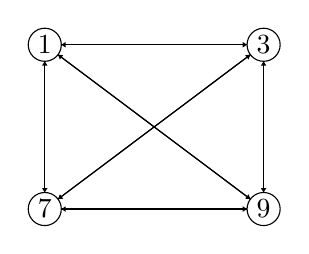
\begin{tikzpicture}[scale=0.07]
\tikzstyle{every node}+=[inner sep=0pt]
\draw [black] (18.7,-9.6) circle (3);
\draw (18.7,-9.6) node {$1$};
\draw [black] (58.4,-9.6) circle (3);
\draw (58.4,-9.6) node {$3$};
\draw [black] (18.7,-39.4) circle (3);
\draw (18.7,-39.4) node {$7$};
\draw [black] (58.4,-39.4) circle (3);
\draw (58.4,-39.4) node {$9$};
\draw [black] (21.7,-9.6) -- (55.4,-9.6);
\fill [black] (55.4,-9.6) -- (54.6,-9.1) -- (54.6,-10.1);
\draw [black] (55.4,-9.6) -- (21.7,-9.6);
\fill [black] (21.7,-9.6) -- (22.5,-10.1) -- (22.5,-9.1);
\draw [black] (21.1,-11.4) -- (56,-37.6);
\fill [black] (56,-37.6) -- (55.66,-36.72) -- (55.06,-37.52);
\draw [black] (56,-37.6) -- (21.1,-11.4);
\fill [black] (21.1,-11.4) -- (21.44,-12.28) -- (22.04,-11.48);
\draw [black] (58.4,-36.4) -- (58.4,-12.6);
\fill [black] (58.4,-12.6) -- (57.9,-13.4) -- (58.9,-13.4);
\draw [black] (58.4,-12.6) -- (58.4,-36.4);
\fill [black] (58.4,-36.4) -- (58.9,-35.6) -- (57.9,-35.6);
\draw [black] (21.7,-39.4) -- (55.4,-39.4);
\fill [black] (55.4,-39.4) -- (54.6,-38.9) -- (54.6,-39.9);
\draw [black] (55.4,-39.4) -- (21.7,-39.4);
\fill [black] (21.7,-39.4) -- (22.5,-39.9) -- (22.5,-38.9);
\draw [black] (56,-11.4) -- (21.1,-37.6);
\fill [black] (21.1,-37.6) -- (22.04,-37.52) -- (21.44,-36.72);
\draw [black] (21.1,-37.6) -- (56,-11.4);
\fill [black] (56,-11.4) -- (55.06,-11.48) -- (55.66,-12.28);
\draw [black] (18.7,-12.6) -- (18.7,-36.4);
\fill [black] (18.7,-36.4) -- (19.2,-35.6) -- (18.2,-35.6);
\draw [black] (18.7,-36.4) -- (18.7,-12.6);
\fill [black] (18.7,-12.6) -- (18.2,-13.4) -- (19.2,-13.4);
\end{tikzpicture}
\end{center}



\begin{center}
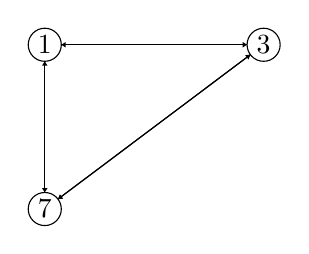
\begin{tikzpicture}[scale=0.07]
\tikzstyle{every node}+=[inner sep=0pt]
\draw [black] (18.7,-9.6) circle (3);
\draw (18.7,-9.6) node {$1$};
\draw [black] (58.4,-9.6) circle (3);
\draw (58.4,-9.6) node {$3$};
\draw [black] (18.7,-39.4) circle (3);
\draw (18.7,-39.4) node {$7$};
\draw [black] (21.7,-9.6) -- (55.4,-9.6);
\fill [black] (55.4,-9.6) -- (54.6,-9.1) -- (54.6,-10.1);
\draw [black] (55.4,-9.6) -- (21.7,-9.6);
\fill [black] (21.7,-9.6) -- (22.5,-10.1) -- (22.5,-9.1);
\draw [black] (56,-11.4) -- (21.1,-37.6);
\fill [black] (21.1,-37.6) -- (22.04,-37.52) -- (21.44,-36.72);
\draw [black] (21.1,-37.6) -- (56,-11.4);
\fill [black] (56,-11.4) -- (55.06,-11.48) -- (55.66,-12.28);
\draw [black] (18.7,-12.6) -- (18.7,-36.4);
\fill [black] (18.7,-36.4) -- (19.2,-35.6) -- (18.2,-35.6);
\draw [black] (18.7,-36.4) -- (18.7,-12.6);
\fill [black] (18.7,-12.6) -- (18.2,-13.4) -- (19.2,-13.4);
\end{tikzpicture}
\end{center}



\begin{center}
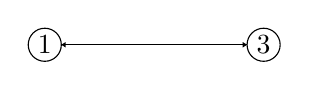
\begin{tikzpicture}[scale=0.07]
\tikzstyle{every node}+=[inner sep=0pt]
\draw [black] (18.7,-9.6) circle (3);
\draw (18.7,-9.6) node {$1$};
\draw [black] (58.4,-9.6) circle (3);
\draw (58.4,-9.6) node {$3$};
\draw [black] (21.7,-9.6) -- (55.4,-9.6);
\fill [black] (55.4,-9.6) -- (54.6,-9.1) -- (54.6,-10.1);
\draw [black] (55.4,-9.6) -- (21.7,-9.6);
\fill [black] (21.7,-9.6) -- (22.5,-10.1) -- (22.5,-9.1);
\end{tikzpicture}
\end{center}


\begin{center}
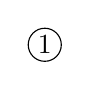
\begin{tikzpicture}[scale=0.07]
\tikzstyle{every node}+=[inner sep=0pt]
\draw [black] (18.7,-9.6) circle (3);
\draw (18.7,-9.6) node {$1$};
\end{tikzpicture}
\end{center}
\newpage








\subsection{}

the maximal elimination clique is only 3. this is the more efficient elimination ordering (probably the minimal one).

\begin{center}
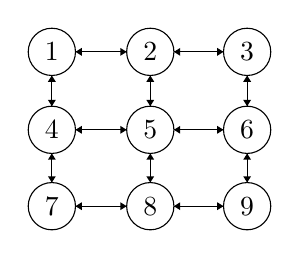
\begin{tikzpicture}[scale=0.1]
\tikzstyle{every node}+=[inner sep=0pt]
\draw [black] (16.3,-15) circle (3);
\draw (16.3,-15) node {$1$};
\draw [black] (28.8,-15) circle (3);
\draw (28.8,-15) node {$2$};
\draw [black] (41.1,-15) circle (3);
\draw (41.1,-15) node {$3$};
\draw [black] (16.3,-24.9) circle (3);
\draw (16.3,-24.9) node {$4$};
\draw [black] (28.8,-24.9) circle (3);
\draw (28.8,-24.9) node {$5$};
\draw [black] (41.1,-24.9) circle (3);
\draw (41.1,-24.9) node {$6$};
\draw [black] (16.3,-34.6) circle (3);
\draw (16.3,-34.6) node {$7$};
\draw [black] (28.8,-34.6) circle (3);
\draw (28.8,-34.6) node {$8$};
\draw [black] (41.1,-34.6) circle (3);
\draw (41.1,-34.6) node {$9$};
\draw [black] (19.3,-15) -- (25.8,-15);
\fill [black] (25.8,-15) -- (25,-14.5) -- (25,-15.5);
\draw [black] (25.8,-15) -- (19.3,-15);
\fill [black] (19.3,-15) -- (20.1,-15.5) -- (20.1,-14.5);
\draw [black] (16.3,-18) -- (16.3,-21.9);
\fill [black] (16.3,-21.9) -- (16.8,-21.1) -- (15.8,-21.1);
\draw [black] (16.3,-21.9) -- (16.3,-18);
\fill [black] (16.3,-18) -- (15.8,-18.8) -- (16.8,-18.8);
\draw [black] (16.3,-27.9) -- (16.3,-31.6);
\fill [black] (16.3,-31.6) -- (16.8,-30.8) -- (15.8,-30.8);
\draw [black] (16.3,-31.6) -- (16.3,-27.9);
\fill [black] (16.3,-27.9) -- (15.8,-28.7) -- (16.8,-28.7);
\draw [black] (19.3,-24.9) -- (25.8,-24.9);
\fill [black] (25.8,-24.9) -- (25,-24.4) -- (25,-25.4);
\draw [black] (25.8,-24.9) -- (19.3,-24.9);
\fill [black] (19.3,-24.9) -- (20.1,-25.4) -- (20.1,-24.4);
\draw [black] (19.3,-34.6) -- (25.8,-34.6);
\fill [black] (25.8,-34.6) -- (25,-34.1) -- (25,-35.1);
\draw [black] (25.8,-34.6) -- (19.3,-34.6);
\fill [black] (19.3,-34.6) -- (20.1,-35.1) -- (20.1,-34.1);
\draw [black] (31.8,-34.6) -- (38.1,-34.6);
\fill [black] (38.1,-34.6) -- (37.3,-34.1) -- (37.3,-35.1);
\draw [black] (38.1,-34.6) -- (31.8,-34.6);
\fill [black] (31.8,-34.6) -- (32.6,-35.1) -- (32.6,-34.1);
\draw [black] (28.8,-31.6) -- (28.8,-27.9);
\fill [black] (28.8,-27.9) -- (28.3,-28.7) -- (29.3,-28.7);
\draw [black] (28.8,-27.9) -- (28.8,-31.6);
\fill [black] (28.8,-31.6) -- (29.3,-30.8) -- (28.3,-30.8);
\draw [black] (28.8,-21.9) -- (28.8,-18);
\fill [black] (28.8,-18) -- (28.3,-18.8) -- (29.3,-18.8);
\draw [black] (28.8,-18) -- (28.8,-21.9);
\fill [black] (28.8,-21.9) -- (29.3,-21.1) -- (28.3,-21.1);
\draw [black] (31.8,-15) -- (38.1,-15);
\fill [black] (38.1,-15) -- (37.3,-14.5) -- (37.3,-15.5);
\draw [black] (38.1,-15) -- (31.8,-15);
\fill [black] (31.8,-15) -- (32.6,-15.5) -- (32.6,-14.5);
\draw [black] (41.1,-21.9) -- (41.1,-18);
\fill [black] (41.1,-18) -- (40.6,-18.8) -- (41.6,-18.8);
\draw [black] (41.1,-18) -- (41.1,-21.9);
\fill [black] (41.1,-21.9) -- (41.6,-21.1) -- (40.6,-21.1);
\draw [black] (41.1,-27.9) -- (41.1,-31.6);
\fill [black] (41.1,-31.6) -- (41.6,-30.8) -- (40.6,-30.8);
\draw [black] (41.1,-31.6) -- (41.1,-27.9);
\fill [black] (41.1,-27.9) -- (40.6,-28.7) -- (41.6,-28.7);
\draw [black] (38.1,-24.9) -- (31.8,-24.9);
\fill [black] (31.8,-24.9) -- (32.6,-25.4) -- (32.6,-24.4);
\draw [black] (31.8,-24.9) -- (38.1,-24.9);
\fill [black] (38.1,-24.9) -- (37.3,-24.4) -- (37.3,-25.4);
\end{tikzpicture}
\end{center}


\begin{center}
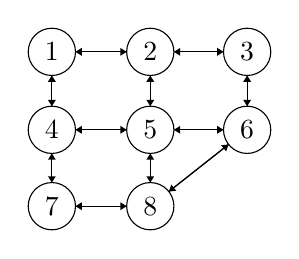
\begin{tikzpicture}[scale=0.1]
\tikzstyle{every node}+=[inner sep=0pt]
\draw [black] (16.3,-15) circle (3);
\draw (16.3,-15) node {$1$};
\draw [black] (28.8,-15) circle (3);
\draw (28.8,-15) node {$2$};
\draw [black] (41.1,-15) circle (3);
\draw (41.1,-15) node {$3$};
\draw [black] (16.3,-24.9) circle (3);
\draw (16.3,-24.9) node {$4$};
\draw [black] (28.8,-24.9) circle (3);
\draw (28.8,-24.9) node {$5$};
\draw [black] (41.1,-24.9) circle (3);
\draw (41.1,-24.9) node {$6$};
\draw [black] (16.3,-34.6) circle (3);
\draw (16.3,-34.6) node {$7$};
\draw [black] (28.8,-34.6) circle (3);
\draw (28.8,-34.6) node {$8$};
\draw [black] (19.3,-15) -- (25.8,-15);
\fill [black] (25.8,-15) -- (25,-14.5) -- (25,-15.5);
\draw [black] (25.8,-15) -- (19.3,-15);
\fill [black] (19.3,-15) -- (20.1,-15.5) -- (20.1,-14.5);
\draw [black] (16.3,-18) -- (16.3,-21.9);
\fill [black] (16.3,-21.9) -- (16.8,-21.1) -- (15.8,-21.1);
\draw [black] (16.3,-21.9) -- (16.3,-18);
\fill [black] (16.3,-18) -- (15.8,-18.8) -- (16.8,-18.8);
\draw [black] (16.3,-27.9) -- (16.3,-31.6);
\fill [black] (16.3,-31.6) -- (16.8,-30.8) -- (15.8,-30.8);
\draw [black] (16.3,-31.6) -- (16.3,-27.9);
\fill [black] (16.3,-27.9) -- (15.8,-28.7) -- (16.8,-28.7);
\draw [black] (19.3,-24.9) -- (25.8,-24.9);
\fill [black] (25.8,-24.9) -- (25,-24.4) -- (25,-25.4);
\draw [black] (25.8,-24.9) -- (19.3,-24.9);
\fill [black] (19.3,-24.9) -- (20.1,-25.4) -- (20.1,-24.4);
\draw [black] (19.3,-34.6) -- (25.8,-34.6);
\fill [black] (25.8,-34.6) -- (25,-34.1) -- (25,-35.1);
\draw [black] (25.8,-34.6) -- (19.3,-34.6);
\fill [black] (19.3,-34.6) -- (20.1,-35.1) -- (20.1,-34.1);
\draw [black] (28.8,-31.6) -- (28.8,-27.9);
\fill [black] (28.8,-27.9) -- (28.3,-28.7) -- (29.3,-28.7);
\draw [black] (28.8,-27.9) -- (28.8,-31.6);
\fill [black] (28.8,-31.6) -- (29.3,-30.8) -- (28.3,-30.8);
\draw [black] (28.8,-21.9) -- (28.8,-18);
\fill [black] (28.8,-18) -- (28.3,-18.8) -- (29.3,-18.8);
\draw [black] (28.8,-18) -- (28.8,-21.9);
\fill [black] (28.8,-21.9) -- (29.3,-21.1) -- (28.3,-21.1);
\draw [black] (31.8,-15) -- (38.1,-15);
\fill [black] (38.1,-15) -- (37.3,-14.5) -- (37.3,-15.5);
\draw [black] (38.1,-15) -- (31.8,-15);
\fill [black] (31.8,-15) -- (32.6,-15.5) -- (32.6,-14.5);
\draw [black] (41.1,-21.9) -- (41.1,-18);
\fill [black] (41.1,-18) -- (40.6,-18.8) -- (41.6,-18.8);
\draw [black] (41.1,-18) -- (41.1,-21.9);
\fill [black] (41.1,-21.9) -- (41.6,-21.1) -- (40.6,-21.1);
\draw [black] (38.1,-24.9) -- (31.8,-24.9);
\fill [black] (31.8,-24.9) -- (32.6,-25.4) -- (32.6,-24.4);
\draw [black] (31.8,-24.9) -- (38.1,-24.9);
\fill [black] (38.1,-24.9) -- (37.3,-24.4) -- (37.3,-25.4);
\draw [black] (31.16,-32.74) -- (38.74,-26.76);
\fill [black] (38.74,-26.76) -- (37.81,-26.86) -- (38.43,-27.65);
\draw [black] (38.74,-26.76) -- (31.16,-32.74);
\fill [black] (31.16,-32.74) -- (32.09,-32.64) -- (31.47,-31.85);
\end{tikzpicture}
\end{center}



\begin{center}
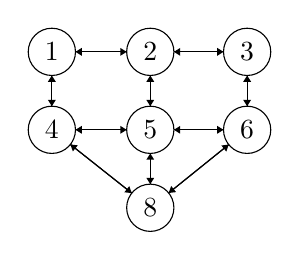
\begin{tikzpicture}[scale=0.1]
\tikzstyle{every node}+=[inner sep=0pt]
\draw [black] (16.3,-15) circle (3);
\draw (16.3,-15) node {$1$};
\draw [black] (28.8,-15) circle (3);
\draw (28.8,-15) node {$2$};
\draw [black] (41.1,-15) circle (3);
\draw (41.1,-15) node {$3$};
\draw [black] (16.3,-24.9) circle (3);
\draw (16.3,-24.9) node {$4$};
\draw [black] (28.8,-24.9) circle (3);
\draw (28.8,-24.9) node {$5$};
\draw [black] (41.1,-24.9) circle (3);
\draw (41.1,-24.9) node {$6$};
\draw [black] (28.8,-34.8) circle (3);
\draw (28.8,-34.8) node {$8$};
\draw [black] (19.3,-15) -- (25.8,-15);
\fill [black] (25.8,-15) -- (25,-14.5) -- (25,-15.5);
\draw [black] (25.8,-15) -- (19.3,-15);
\fill [black] (19.3,-15) -- (20.1,-15.5) -- (20.1,-14.5);
\draw [black] (16.3,-18) -- (16.3,-21.9);
\fill [black] (16.3,-21.9) -- (16.8,-21.1) -- (15.8,-21.1);
\draw [black] (16.3,-21.9) -- (16.3,-18);
\fill [black] (16.3,-18) -- (15.8,-18.8) -- (16.8,-18.8);
\draw [black] (19.3,-24.9) -- (25.8,-24.9);
\fill [black] (25.8,-24.9) -- (25,-24.4) -- (25,-25.4);
\draw [black] (25.8,-24.9) -- (19.3,-24.9);
\fill [black] (19.3,-24.9) -- (20.1,-25.4) -- (20.1,-24.4);
\draw [black] (28.8,-31.8) -- (28.8,-27.9);
\fill [black] (28.8,-27.9) -- (28.3,-28.7) -- (29.3,-28.7);
\draw [black] (28.8,-27.9) -- (28.8,-31.8);
\fill [black] (28.8,-31.8) -- (29.3,-31) -- (28.3,-31);
\draw [black] (28.8,-21.9) -- (28.8,-18);
\fill [black] (28.8,-18) -- (28.3,-18.8) -- (29.3,-18.8);
\draw [black] (28.8,-18) -- (28.8,-21.9);
\fill [black] (28.8,-21.9) -- (29.3,-21.1) -- (28.3,-21.1);
\draw [black] (31.8,-15) -- (38.1,-15);
\fill [black] (38.1,-15) -- (37.3,-14.5) -- (37.3,-15.5);
\draw [black] (38.1,-15) -- (31.8,-15);
\fill [black] (31.8,-15) -- (32.6,-15.5) -- (32.6,-14.5);
\draw [black] (41.1,-21.9) -- (41.1,-18);
\fill [black] (41.1,-18) -- (40.6,-18.8) -- (41.6,-18.8);
\draw [black] (41.1,-18) -- (41.1,-21.9);
\fill [black] (41.1,-21.9) -- (41.6,-21.1) -- (40.6,-21.1);
\draw [black] (38.1,-24.9) -- (31.8,-24.9);
\fill [black] (31.8,-24.9) -- (32.6,-25.4) -- (32.6,-24.4);
\draw [black] (31.8,-24.9) -- (38.1,-24.9);
\fill [black] (38.1,-24.9) -- (37.3,-24.4) -- (37.3,-25.4);
\draw [black] (31.14,-32.92) -- (38.76,-26.78);
\fill [black] (38.76,-26.78) -- (37.83,-26.89) -- (38.45,-27.67);
\draw [black] (38.76,-26.78) -- (31.14,-32.92);
\fill [black] (31.14,-32.92) -- (32.07,-32.81) -- (31.45,-32.03);
\draw [black] (18.65,-26.76) -- (26.45,-32.94);
\fill [black] (26.45,-32.94) -- (26.13,-32.05) -- (25.51,-32.83);
\draw [black] (26.45,-32.94) -- (18.65,-26.76);
\fill [black] (18.65,-26.76) -- (18.97,-27.65) -- (19.59,-26.87);
\end{tikzpicture}
\end{center}


\begin{center}
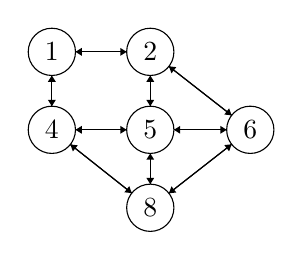
\begin{tikzpicture}[scale=0.1]
\tikzstyle{every node}+=[inner sep=0pt]
\draw [black] (16.3,-15) circle (3);
\draw (16.3,-15) node {$1$};
\draw [black] (28.8,-15) circle (3);
\draw (28.8,-15) node {$2$};
\draw [black] (16.3,-24.9) circle (3);
\draw (16.3,-24.9) node {$4$};
\draw [black] (28.8,-24.9) circle (3);
\draw (28.8,-24.9) node {$5$};
\draw [black] (41.5,-24.9) circle (3);
\draw (41.5,-24.9) node {$6$};
\draw [black] (28.8,-34.8) circle (3);
\draw (28.8,-34.8) node {$8$};
\draw [black] (19.3,-15) -- (25.8,-15);
\fill [black] (25.8,-15) -- (25,-14.5) -- (25,-15.5);
\draw [black] (25.8,-15) -- (19.3,-15);
\fill [black] (19.3,-15) -- (20.1,-15.5) -- (20.1,-14.5);
\draw [black] (16.3,-18) -- (16.3,-21.9);
\fill [black] (16.3,-21.9) -- (16.8,-21.1) -- (15.8,-21.1);
\draw [black] (16.3,-21.9) -- (16.3,-18);
\fill [black] (16.3,-18) -- (15.8,-18.8) -- (16.8,-18.8);
\draw [black] (19.3,-24.9) -- (25.8,-24.9);
\fill [black] (25.8,-24.9) -- (25,-24.4) -- (25,-25.4);
\draw [black] (25.8,-24.9) -- (19.3,-24.9);
\fill [black] (19.3,-24.9) -- (20.1,-25.4) -- (20.1,-24.4);
\draw [black] (28.8,-31.8) -- (28.8,-27.9);
\fill [black] (28.8,-27.9) -- (28.3,-28.7) -- (29.3,-28.7);
\draw [black] (28.8,-27.9) -- (28.8,-31.8);
\fill [black] (28.8,-31.8) -- (29.3,-31) -- (28.3,-31);
\draw [black] (28.8,-21.9) -- (28.8,-18);
\fill [black] (28.8,-18) -- (28.3,-18.8) -- (29.3,-18.8);
\draw [black] (28.8,-18) -- (28.8,-21.9);
\fill [black] (28.8,-21.9) -- (29.3,-21.1) -- (28.3,-21.1);
\draw [black] (38.5,-24.9) -- (31.8,-24.9);
\fill [black] (31.8,-24.9) -- (32.6,-25.4) -- (32.6,-24.4);
\draw [black] (31.8,-24.9) -- (38.5,-24.9);
\fill [black] (38.5,-24.9) -- (37.7,-24.4) -- (37.7,-25.4);
\draw [black] (31.17,-32.96) -- (39.13,-26.74);
\fill [black] (39.13,-26.74) -- (38.2,-26.84) -- (38.81,-27.63);
\draw [black] (39.13,-26.74) -- (31.17,-32.96);
\fill [black] (31.17,-32.96) -- (32.1,-32.86) -- (31.49,-32.07);
\draw [black] (18.65,-26.76) -- (26.45,-32.94);
\fill [black] (26.45,-32.94) -- (26.13,-32.05) -- (25.51,-32.83);
\draw [black] (26.45,-32.94) -- (18.65,-26.76);
\fill [black] (18.65,-26.76) -- (18.97,-27.65) -- (19.59,-26.87);
\draw [black] (39.13,-23.06) -- (31.17,-16.84);
\fill [black] (31.17,-16.84) -- (31.49,-17.73) -- (32.1,-16.94);
\draw [black] (31.17,-16.84) -- (39.13,-23.06);
\fill [black] (39.13,-23.06) -- (38.81,-22.17) -- (38.2,-22.96);
\end{tikzpicture}
\end{center}



\begin{center}
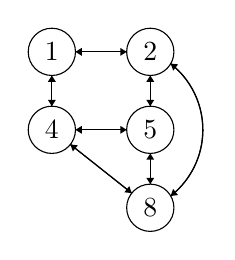
\begin{tikzpicture}[scale=0.1]
\tikzstyle{every node}+=[inner sep=0pt]
\draw [black] (16.3,-15) circle (3);
\draw (16.3,-15) node {$1$};
\draw [black] (28.8,-15) circle (3);
\draw (28.8,-15) node {$2$};
\draw [black] (16.3,-24.9) circle (3);
\draw (16.3,-24.9) node {$4$};
\draw [black] (28.8,-24.9) circle (3);
\draw (28.8,-24.9) node {$5$};
\draw [black] (28.8,-34.8) circle (3);
\draw (28.8,-34.8) node {$8$};
\draw [black] (19.3,-15) -- (25.8,-15);
\fill [black] (25.8,-15) -- (25,-14.5) -- (25,-15.5);
\draw [black] (25.8,-15) -- (19.3,-15);
\fill [black] (19.3,-15) -- (20.1,-15.5) -- (20.1,-14.5);
\draw [black] (16.3,-18) -- (16.3,-21.9);
\fill [black] (16.3,-21.9) -- (16.8,-21.1) -- (15.8,-21.1);
\draw [black] (16.3,-21.9) -- (16.3,-18);
\fill [black] (16.3,-18) -- (15.8,-18.8) -- (16.8,-18.8);
\draw [black] (19.3,-24.9) -- (25.8,-24.9);
\fill [black] (25.8,-24.9) -- (25,-24.4) -- (25,-25.4);
\draw [black] (25.8,-24.9) -- (19.3,-24.9);
\fill [black] (19.3,-24.9) -- (20.1,-25.4) -- (20.1,-24.4);
\draw [black] (28.8,-31.8) -- (28.8,-27.9);
\fill [black] (28.8,-27.9) -- (28.3,-28.7) -- (29.3,-28.7);
\draw [black] (28.8,-27.9) -- (28.8,-31.8);
\fill [black] (28.8,-31.8) -- (29.3,-31) -- (28.3,-31);
\draw [black] (28.8,-21.9) -- (28.8,-18);
\fill [black] (28.8,-18) -- (28.3,-18.8) -- (29.3,-18.8);
\draw [black] (28.8,-18) -- (28.8,-21.9);
\fill [black] (28.8,-21.9) -- (29.3,-21.1) -- (28.3,-21.1);
\draw [black] (18.65,-26.76) -- (26.45,-32.94);
\fill [black] (26.45,-32.94) -- (26.13,-32.05) -- (25.51,-32.83);
\draw [black] (26.45,-32.94) -- (18.65,-26.76);
\fill [black] (18.65,-26.76) -- (18.97,-27.65) -- (19.59,-26.87);
\draw [black] (31.385,-16.503) arc (51.78382:-51.78382:10.688);
\fill [black] (31.38,-33.3) -- (32.32,-33.19) -- (31.7,-32.41);
\draw [black] (31.391,-16.493) arc (51.99175:-51.99175:10.67);
\fill [black] (31.39,-16.49) -- (31.71,-17.38) -- (32.33,-16.59);
\end{tikzpicture}
\end{center}



\begin{center}
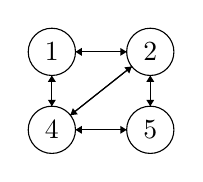
\begin{tikzpicture}[scale=0.1]
\tikzstyle{every node}+=[inner sep=0pt]
\draw [black] (16.3,-15) circle (3);
\draw (16.3,-15) node {$1$};
\draw [black] (28.8,-15) circle (3);
\draw (28.8,-15) node {$2$};
\draw [black] (16.3,-24.9) circle (3);
\draw (16.3,-24.9) node {$4$};
\draw [black] (28.8,-24.9) circle (3);
\draw (28.8,-24.9) node {$5$};
\draw [black] (19.3,-15) -- (25.8,-15);
\fill [black] (25.8,-15) -- (25,-14.5) -- (25,-15.5);
\draw [black] (25.8,-15) -- (19.3,-15);
\fill [black] (19.3,-15) -- (20.1,-15.5) -- (20.1,-14.5);
\draw [black] (16.3,-18) -- (16.3,-21.9);
\fill [black] (16.3,-21.9) -- (16.8,-21.1) -- (15.8,-21.1);
\draw [black] (16.3,-21.9) -- (16.3,-18);
\fill [black] (16.3,-18) -- (15.8,-18.8) -- (16.8,-18.8);
\draw [black] (19.3,-24.9) -- (25.8,-24.9);
\fill [black] (25.8,-24.9) -- (25,-24.4) -- (25,-25.4);
\draw [black] (25.8,-24.9) -- (19.3,-24.9);
\fill [black] (19.3,-24.9) -- (20.1,-25.4) -- (20.1,-24.4);
\draw [black] (28.8,-21.9) -- (28.8,-18);
\fill [black] (28.8,-18) -- (28.3,-18.8) -- (29.3,-18.8);
\draw [black] (28.8,-18) -- (28.8,-21.9);
\fill [black] (28.8,-21.9) -- (29.3,-21.1) -- (28.3,-21.1);
\draw [black] (26.45,-16.86) -- (18.65,-23.04);
\fill [black] (18.65,-23.04) -- (19.59,-22.93) -- (18.97,-22.15);
\draw [black] (18.65,-23.04) -- (26.45,-16.86);
\fill [black] (26.45,-16.86) -- (25.51,-16.97) -- (26.13,-17.75);
\end{tikzpicture}
\end{center}


\begin{center}
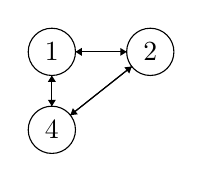
\begin{tikzpicture}[scale=0.1]
\tikzstyle{every node}+=[inner sep=0pt]
\draw [black] (16.3,-15) circle (3);
\draw (16.3,-15) node {$1$};
\draw [black] (28.8,-15) circle (3);
\draw (28.8,-15) node {$2$};
\draw [black] (16.3,-24.9) circle (3);
\draw (16.3,-24.9) node {$4$};
\draw [black] (19.3,-15) -- (25.8,-15);
\fill [black] (25.8,-15) -- (25,-14.5) -- (25,-15.5);
\draw [black] (25.8,-15) -- (19.3,-15);
\fill [black] (19.3,-15) -- (20.1,-15.5) -- (20.1,-14.5);
\draw [black] (16.3,-18) -- (16.3,-21.9);
\fill [black] (16.3,-21.9) -- (16.8,-21.1) -- (15.8,-21.1);
\draw [black] (16.3,-21.9) -- (16.3,-18);
\fill [black] (16.3,-18) -- (15.8,-18.8) -- (16.8,-18.8);
\draw [black] (26.45,-16.86) -- (18.65,-23.04);
\fill [black] (18.65,-23.04) -- (19.59,-22.93) -- (18.97,-22.15);
\draw [black] (18.65,-23.04) -- (26.45,-16.86);
\fill [black] (26.45,-16.86) -- (25.51,-16.97) -- (26.13,-17.75);
\end{tikzpicture}
\end{center}


\begin{center}
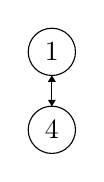
\begin{tikzpicture}[scale=0.1]
\tikzstyle{every node}+=[inner sep=0pt]
\draw [black] (16.3,-15) circle (3);
\draw (16.3,-15) node {$1$};
\draw [black] (16.3,-24.9) circle (3);
\draw (16.3,-24.9) node {$4$};
\draw [black] (16.3,-18) -- (16.3,-21.9);
\fill [black] (16.3,-21.9) -- (16.8,-21.1) -- (15.8,-21.1);
\draw [black] (16.3,-21.9) -- (16.3,-18);
\fill [black] (16.3,-18) -- (15.8,-18.8) -- (16.8,-18.8);
\end{tikzpicture}
\end{center}

\begin{center}
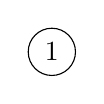
\begin{tikzpicture}[scale=0.1]
\tikzstyle{every node}+=[inner sep=0pt]
\draw [black] (16.3,-15) circle (3);
\draw (16.3,-15) node {$1$};
\end{tikzpicture}
\end{center}



%TODO
%\end{comment}



\newpage
\subsection{}
\paragraph{}
$n^2$ would be trivially true as it about the tree width of an $n \times n$ clique. assuming the elimination ordering of (3b) is optimal or near optimal (which should be the point, as it works in from the lower-degree corners and edges), there are only $3-$cliques. also, the maximal clique of the minimal elimination ordering of a $2 \times 2$ grid is $3$ (by symmetry every elimination ordering is isomorphic). i played around with a $4 \times 4$ grid but i couldn't reduce by some optimal elimination ordering to a $3 \times 3$. i also tried to see if i could find an elimination ordering for the $4 \times 4$ that preserves a constant 3 clique, by working in from�(i.e. eliminating first) the corners and edges; or row-by-row and col-by-col. but i saw $4-$cliques. however, i can't prove either that this was a $minimal$ elimination ordering or a $maximal$ clique (the "minimax" definition of treewidth). it's probably the minimal elimination ordering, but it might not be the maximal elimination clique. the treewidth could be (unlikely) some $O(n)$ or (even less likely) a const $3-1$.


\paragraph{}
thus, i say the treewidth of an $n \times n$ grid graph is $n-1$ as i think  the maximal elimination clique of the minimal elimination ordering is $n$.










\end{document}
